\documentclass[12pt,a4paper]{article}

\usepackage[utf8]{inputenc}
\usepackage{amsmath}
\usepackage{amsfonts}
\usepackage{makeidx}
\usepackage{amssymb}
\usepackage{hyperref}
\usepackage{graphicx}
\usepackage{caption}
\usepackage{float}
\usepackage{indentfirst}
% \usepackage[spanish,es-tabla]{babel}


\captionsetup[figure]{font=small,skip=-5pt}

\title{Sistemas de Inteligencia Artificial\\Redes Neuronales\\Trabajo Práctico Especial Número 2}
\date{Mayo 2015}
\author{Federico Tedin - 53048\\Javier Fraire - 53023\\Ignacio Rivera - 53029}

\makeindex

\begin{document}
\maketitle
\thispagestyle{empty}

\vspace{5mm}
\renewcommand{\abstractname}{Resumen:}
\begin{abstract}

\centering
Implementar una red neuronal multicapa con aprendizaje supervisado con la cual se resuelva el siguiente problema:
$$ y = sin(x)x^3 + \frac{x}{2} $$
\end{abstract}

\clearpage

\renewcommand{\contentsname}{Índice}
\tableofcontents
\thispagestyle{empty}
\clearpage
\setcounter{page}{1}


\section{Introducción}
\subsection{Objetivo}

El objetivo del trabajo práctico realizado fue diseñar una red neuronal que logre estimar una función $f(x)$ definida sobre números reales.  La función utilizada en éste trabajo fue la siguiente:

$$ f(x) = sin(x)x^3 + \frac{x}{2}, \ \text{con} \ x \ \epsilon \ [10, 45] $$

La representación gráfica de la función se puede observar en la figura \ref{fig:fx} del anexo.

\subsection{Contexto}

El trabajo práctico fue realizado utilizando \emph{Python 3.4}.  Se utilizó la librería \emph{numpy 1.8.2} para poder realizar las operaciones matemáticas necesarias, y la librería \emph{matplotlib\ 1.4.2} para crear los gráficos.

\subsection{Aclaraciones}

Cuando se especifique la arquitectura (\emph{arq}) de una red en éste informe, se omitirá siempre la ultima capa (capa de salida), que siempre tendrá una sola neurona.  Por ejemplo, la arquitectura $20-5$ consiste en veinte neuronas en la primera capa, cinco en la segunda, y una en la última capa.

Cuando se especifique un rango de valores (intervalo), se escribirá de la forma $(a, b, c)$, donde $a$ es el valor mínimo, $b$ el valor máximo, y $c$ la separación entre cada valor del intervalo.

La función de activación será referida como la función $g$.  La $g$ de la capa de salida utilizada siempre será la función lineal. En todas las redes presentadas $\beta$ en las funciones de activación es $1$ en la función tangente hiperbólica y $\frac{1}{2}$ en la función exponencial.

En todas las redes se utilizó \emph{incremental} ya que es más preciso que \emph{batch} que es más probable que alcance mínimos locales.

En las figuras se utilizó el mejor entrenamiento de la red mientras que en la tabla el promedio.

\section{Metodología}	
\subsection{Implementación}

La implementación del proyecto consiste principalmente en dos archivos de código: \emph{layer.py} y \emph{network.py}.  El primer archivo contiene la representación de una capa de la red en código \emph{Python}.  La clase contiene información de la cantidad de entradas y salidas, una referencia a la capa anterior, las entradas, pesos, y la función de activación.  El segundo archivo contiene la representación de la red neuronal en general.  La representación consiste en una clase que cuenta con una lista de capas, salidas esperadas, y varios parámetros adicionales, como por ejemplo la tasa de aprendizaje.  La clase \emph{Network} también se encarga de llevar a cabo el proceso de aprendizaje.

Con los dos archivos mencionados, se logró representar una red neuronal multicapa \emph{feed-forward} con función de activación y parámetros modificables.  El aprendizaje de la red se realizó utilizando el método de \emph{back-propagation}, con las variantes \emph{batch} e \emph{incremental}.  La red entonces fue presentada con una serie de valores uniformemente distribuidos en el intervalo especificado por la cátedra, y con los valores asociados esperados ($f(x)$).  A partir de éstos valores, se comenzó el aprendizaje de la red, y se monitorearon valores como el error cuadrático medio y la cantidad de épocas pasadas, entre otros.

\subsection{Procedimiento}

Para cada prueba, se dividió cada valor del intervalo por el valor de mayor módulo de todos los números del intervalo evaluados en $f$, con el propósito de evitar operar con números de módulo elevado ya que las funciones de activación se encuentran en el rango $[-1,1]$.  De ésta forma, también se logró acercar los valores devueltos por la función $f$ al rango de valores devueltos por la funciones de activación.

\subsubsection{Pruebas Iniciales}

La primera prueba de aprendizaje se realizó con los siguientes parámetros: $arq: 20-5,\ \eta=0.01,\ rango=(10, 45, 0.5),\ g=tanh$.  Los resultados de la prueba se pueden observar en la figura \ref{fig:test1}.  Éstos resultados fueron obtenidos luego de un aprendizaje de 10000 épocas.  Como se puede ver, la función no fue estimada de forma satisfactoria, con un error cuadrático medio final de $E=1.15 \times 10^{-1}$.  El error además permaneció oscilando alrededor del valor 0.1155, como se puede observar en la figura \ref{fig:test1err}.

\subsubsection{Variantes de Arquitectura y Tasa de Aprendizaje}

Los primeros ajustes realizados a la red neuronal fueron el cambio de arquitectura (capas y cantidad de neuronas), y el cambio de la tasa de aprendizaje, $\eta$.

La segunda prueba, entonces, se realizó con los siguiente parámetros: $arq: 62-62-32-16-2,\ \eta=3\times 10^{-5},\ rango=(10, 45, 0.5),\ g=tanh$.  Las diferencias con la prueba anterior entonces fueron el uso de una arquitectura completamente distinta, y un $\eta$ de órdenes de magnitud más pequeño.  Los resultados obtenidos en ésta prueba se pueden observar en la figura \ref{fig:test2}.  Como se puede ver, la función no fue aproximada correctamente debido a la saturación de una gran cantidad de neuronas.

Como se puede observar en las figuras \ref{fig:test1}, \ref{fig:test2}, \ref{fig:test3},\ref{fig:test4} y \ref{fig:test5} en ningún caso se encontró una arquitectura adecuada que pueda estimar la función. En todos los casos el error se estancaba y comenzaba a oscilar alrededor de un determinado valor. Se probaron una gran cantidad de arquitecturas, pero en todas ellas se producía una saturación de las neuronas. También se puede observar que se han probado arquitecturas con una gran cantidad de nodos, para evitar la saturación, pero ésta medida también resultó inefectiva. Sin embrago, esto no significa que no haya una arquitectura adecuada, si no que simplemente no pudo ser hallada en éste contexto de pruebas.

\subsubsection{Variantes del dominio de la función}

Como se mencionó en la sección anterior, no se pudo encontrar ninguna forma de estimar adecuadamente la función en el rango $[10,45]$, por lo que se procedió a probar con el rango $[10, 15]$ con un incremento de $0.1$. En la \emph{Tabla 1} se pueden ver los resultados obtenidos con los distintos parámetros en este rango. También se probaron otros dominios, pero no se pudieron estimar adecuadamente. Vale destacar que antes de tomar ésta decisión, se revisó meticulosamente el algoritmo para determinar si había algún error, pero no se encontró ninguno. Por lo tanto, se probó el algoritmo con otras funciones para obtener una mayor cantidad de resultados. Éstos se pueden apreciar en las figuras \ref{fig:ecuacion1}, \ref{fig:ecuacion2} y \ref{fig:ecuacion3}.

\subsubsection{Pruebas con las distintas funciones de activación}

Se utilizaron tres arquitecturas distintas utilizando las dos funciones de activación. Las arquitecturas se explicaran en detalle más adelante. Como se puede observar en las figuras \ref{fig:test10-15-exp-fn-100}, \ref{fig:test10-15-exp-fn-25}, \ref{fig:test10-15-exp-fn-32} (función exponencial) y en las figuras \ref{fig:test10-15-tanh-fn-100}, \ref{fig:test10-15-tanh-fn-25} y \ref{fig:test10-15-tanh-fn-32} (función tangente hiperbólica) y en la \emph{Tabla 1}, la función tangente hiperbólica obtuvo mejores resultados, en algunos casos obteniendo un error de un orden de magnitud menor entrenando $\frac{1}{10}$ de épocas que la función exponencial. Ésto se puede deber a que la función esta normalizada al rango $[-1, 1]$, el cual coincide con la imagen de la función tangente hiperbólica. Como la función exponencial posee una imagen $[0,1]$, tiene mayores dificultades al estimar la función.

\subsubsection{Variantes de Arquitectura y Tasa de Aprendizaje para el dominio elegido}

Se probaron varias arquitecturas pero finalmente se utilizaron tres para compararlas. Cada arquitectura fue probada con distintas tasas de aprendizaje. Las arquitecturas son:  $32-16-16$, $25-10$ y $100$. Como se puede observar entre las figuras \ref{fig:test10-15-exp-fn-100} y \ref{fig:test10-15-tanh-error-32}, la mejor arquitectura fue la primera. Ésta resultó obtener, en una cantidad menor de épocas, un error menor a $1\times10^{-4}$ (el cual se utilizó como condición de corte). A su vez, $100$ fue la peor arquitectura utilizada ya que no consiguió obtener un error menor a $1\times10^{-4}$ en $50000$ (la máxima cantidad de épocas fijada para este dominio). Ésto se debe también a que ésta tiene una gran cantidad de neuronas y a que utiliza un $\eta$ menor que las otras arquitecturas, lo cual puede causar que el error tenga un declive más lento. Se intentaron utilizar otras configuraciones con menos neuronas, pero éstas se saturaban. También se intentó usar un $\eta$ más pequeño en la arquitectura $100$ pero la red se estancaba en un mínimo local, ya que una tasa de aprendizaje menor implica que el error oscilará más fuertemente.

\subsubsection{Mejoras implementadas}

Las mejoras fueron aplicadas en éste dominio unicaménte a la red óptima. La primer mejora que se implementó fue acotar el valor aleatorio de inicialización  de los pesos a $-\frac{1}{\sqrt[2]{|h_j|}} \leq 0 \leq \frac{1}{\sqrt[2]{|h_j|}}$, donde $|h_j|$ es la cantidad de entradas que tiene una red. Ésto se llevó a cabo ya que la inicialización de los pesos tiene una gran importancia en como se desenvuelve la red. Ésta mejora se utilizó en todas las redes neuronales.

Las dos grandes mejoras que se implementaron fueron \emph{momentum} y \emph{$\eta$ adaptativo}. La primera consiste en: $\Delta_{pq}(t + 1) = \frac{\delta E}{\Delta_{pq}} + \alpha  \Delta_{pq}(t)$, donde $\Delta_{pq}$ es el peso de la neurona $p$ a $q$, $\alpha$ es una constante entre $0$ y $1$ y $t$ el paso en el que se encuentra el algoritmo. Los resultados de ésta mejora se encuentran en la \emph{Tabla 1}. En ésta se puede observar que la red mejoró utilizando la mejora. Ésto se debe a que ayuda a la red a salir de un \emph{plateau} de la función de activación, sin aumentar las oscilaciones.

La segunda mejora consiste en modificar la tasa de aprendizaje en un determinado $\Delta \eta$ según los cambios en el error cuadrático medio luego de $k$ épocas, si éste disminuye $\Delta \eta = \alpha$ y si este aumenta $\Delta \eta = -\beta \eta$. Además se le agrego una pequeña mejora: consiste en reestablecer los pesos a los valores que tenían $k$ épocas antes. Es decir, volver hacia atrás hasta que se haga un paso que disminuya el error. En la \emph{Tabla 1} se observan los efectos de la mejora. Ésto se debe a que una tasa de aprendizaje puede ser adecuada para un momento, pero no para otro más adelante, por lo que se adapta dicha tasa.

Además, se puede observar que la mejora \emph{$\eta$ adaptativo} funcionó mejor que \emph{momentum}. Ésto se debe a que ajustar la tasa de aprendizaje es más efectivo para evitar mínimos locales que ajustar los pesos. También, por las razones mencionadas anteriormente, utilizar ambas mejoras juntas resultó en una red más eficiente.

\subsubsection{Generalización}

En \emph{Tabla 1}, se pueden hayan las generalizaciones realizadas para la función en el dominio $[10,15]$. En las figuras \ref{fig:test10-15-tanh-fn-32-0.001}, \ref{fig:test10-15-tanh-fn-32-momentum-0.001}, \ref{fig:test10-15-tanh-fn-32-adaptative-0.001} y \ref{fig:test10-15-tanh-fn-32-adaptative-momentum-0.001}, se puede observar el resultado de generalizar tomando un intervalo de $0.001$. Se puede ver que el error cuadrático medio no es superior en grandes cantidades al error cuadrático medio de entrenamiento. 

\section{Conclusiones}

En conclusión, elegir una arquitectura adecuada para resolver un problema es una tarea compleja. Se ha demostrado que mayor cantidad de capas o nodos no implica una red más eficiente. Por ejemplo, la red $32-16-16$ resultó más eficiente que la red $100$, que tiene más nodos. Si bien teóricamente todo problema se puede resolver con dos capas y una cantidad determinada con una, se desconoce dicha configuración, y muchas veces es más fácil encontrar una red neuronal eficiente utilizando más capas.

Además, se ha observado que no es necesario entrenar a una red con todos los patrones que se quieren estimar. Se puede enviar un menor conjunto de patrones, y luego, una vez que la red está entrenada, se puede generalizar utilizando una mayor cantidad de patrones.

\clearpage
\appendix
\renewcommand{\figurename}{Figura}
\section{Anexo}

\begin{figure}[H]
\centering
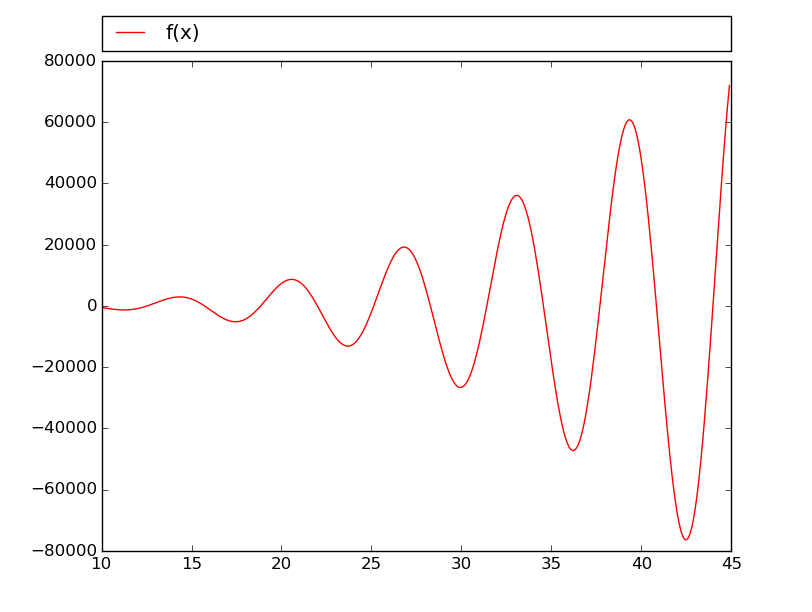
\includegraphics[width=0.85\textwidth]{img/fx.png}
\caption{\label{fig:fx} Función a estimar en el trabajo práctico.}
\end{figure}

\begin{figure}[H]
\centering
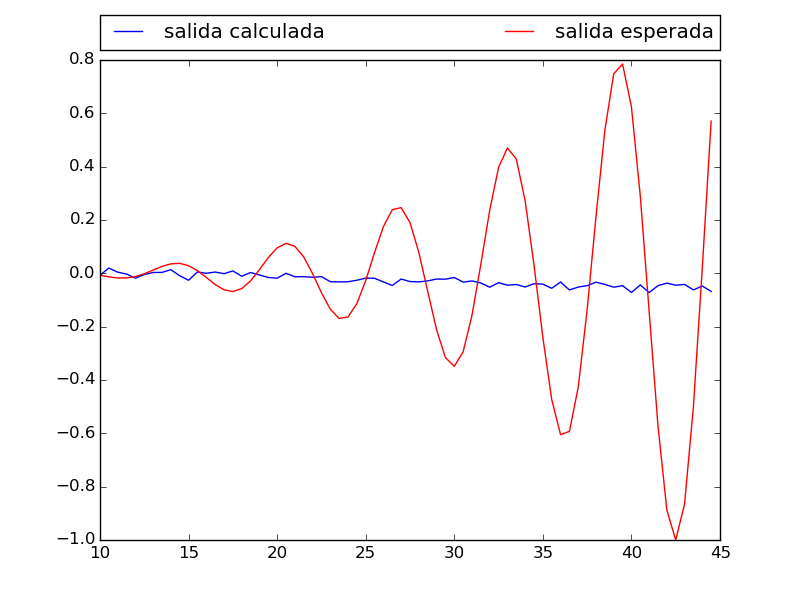
\includegraphics[width=0.85\textwidth]{img/_20__5_-eta_0_01-FUNCTION.png}
\caption{\label{fig:test1} Función. Datos:  $arq: 20-5, \acute{e} pocas \ = 1000,\ \eta = 10^{-2}, \ rango=(10, 45, 0.5),\ g=tanh, \ E = 1.15 \times 10^{-1}$}
\end{figure}

\begin{figure}[H]
\centering
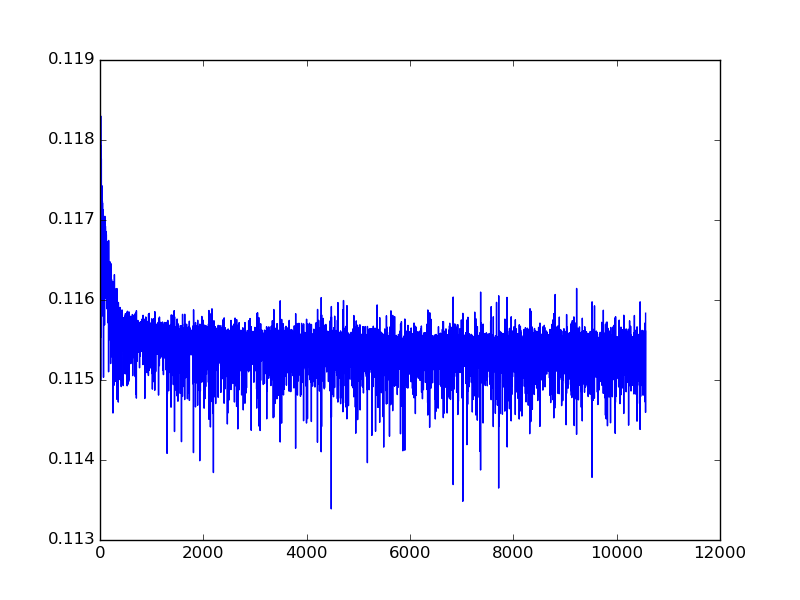
\includegraphics[width=0.85\textwidth]{img/_20__5_-eta_0_01-ERROR.png}
\caption{\label{fig:test1err} Error cuadrático medio. Datos:  $arq: 20-5, \acute{e} pocas \ = 10000,\ \eta = 10^{-2}, \ rango=(10, 45, 0.5),\ g=tanh, \ E = 1.15 \times 10^{-1}$ }
\end{figure}

\begin{figure}[H]
\centering
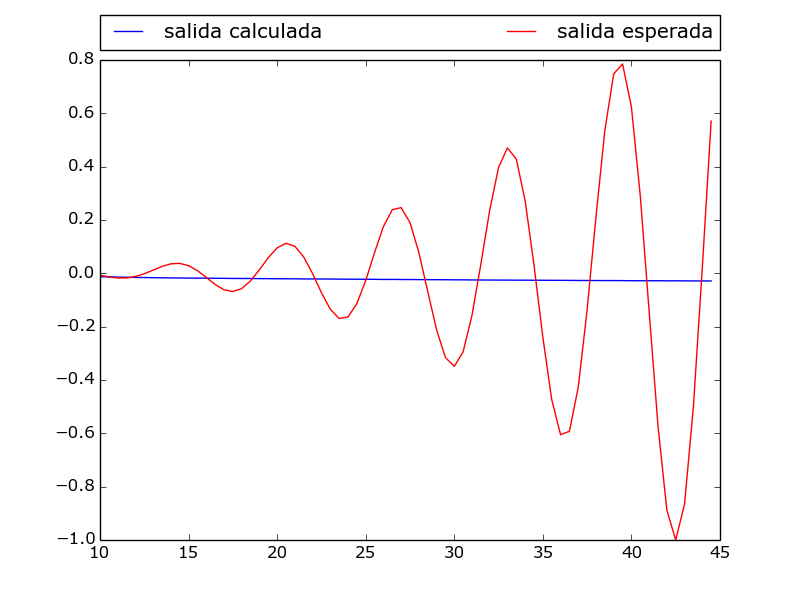
\includegraphics[width=0.85\textwidth]{img/_62__62__32__16__2_-eta_3_0000000000000004e-05-FUNCTION.png}
\caption{\label{fig:test2} Función. Datos:  $arq: 62-62-32-16-2, \acute{e} pocas \ = 2000,\ \eta = 3 \times 10^{-5}, \ rango=(10, 45, 0.5),\ g=tanh, \ E = 1.15 \times 10^{-1}$}
\end{figure}

\begin{figure}[H]
\centering
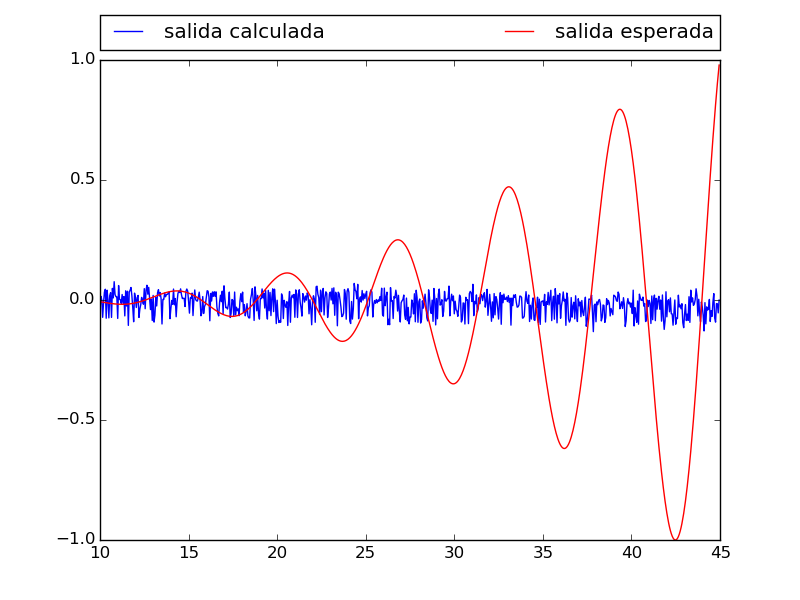
\includegraphics[width=0.85\textwidth]{img/_35_10-eta=001-FUNCTION.png}
\caption{\label{fig:test3} Función. Datos:  $arq: 35-10, \acute{e} pocas \ =19000,\ \eta = 1 \times 10^{-2}, \ rango=(10, 45, 0.05),\ g=tanh, \ E = 1.21 \times 10^{-1}$}
\end{figure}

\begin{figure}[H]
\centering
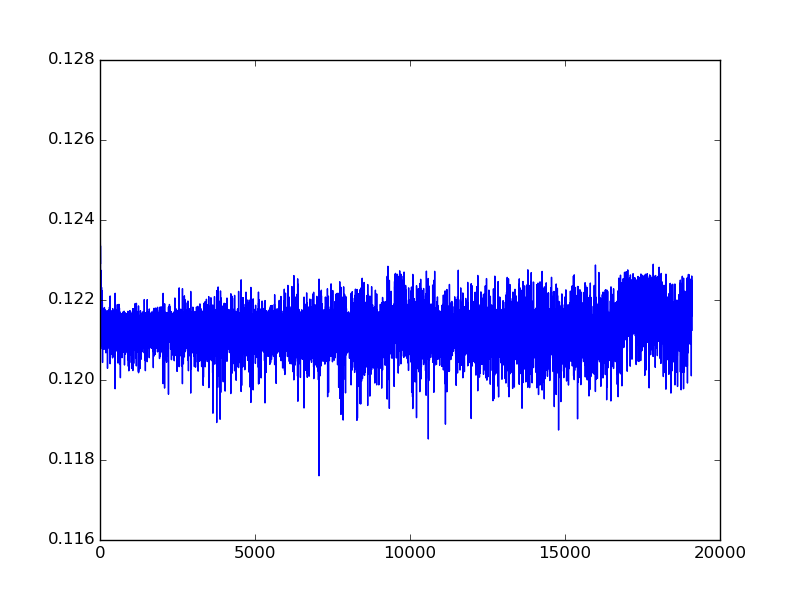
\includegraphics[width=0.85\textwidth]{img/_35_10-eta=001-ERROR.png}
\caption{\label{fig:test3err} Error cuadrático medio. Datos:  $arq: 35-10, \acute{e} pocas \ =19000,\ \eta = 1 \times 10^{-2}, \ rango=(10, 45, 0.05),\ g=tanh, \ E = 1.21 \times 10^{-1}$}
\end{figure}

\begin{figure}[H]
\centering
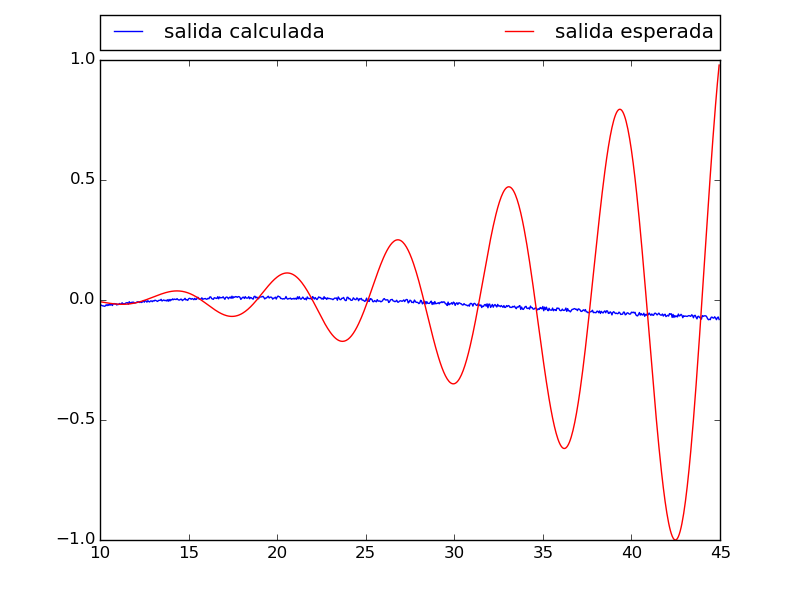
\includegraphics[width=0.85\textwidth]{img/_35_10-eta=00001-FUNCTION.png}
\caption{\label{fig:test4} Función. Datos:  $arq: 35-10, \acute{e} pocas \ =19000,\ \eta = 1 \times 10^{-4}, \ rango=(10, 45, 0.05),\ g=tanh, \ E = 1.21 \times 10^{-1}$}
\end{figure}

\begin{figure}[H]
\centering
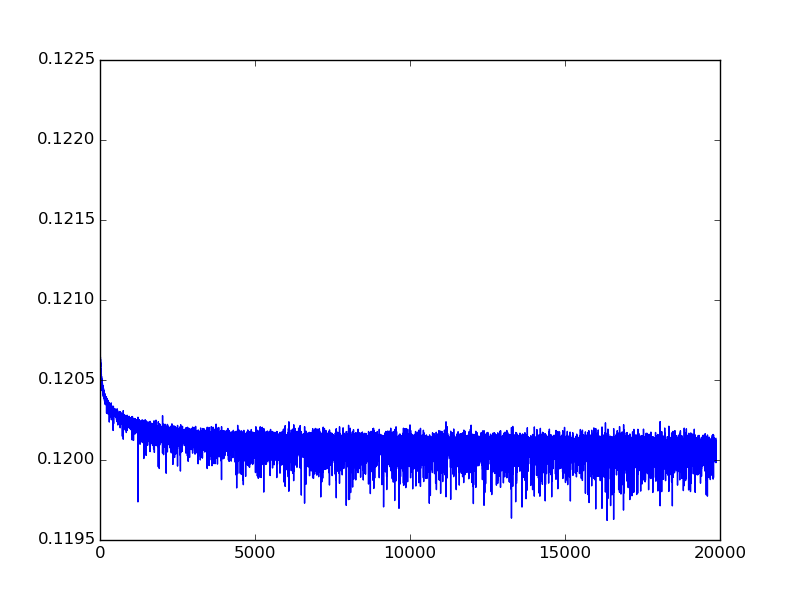
\includegraphics[width=0.85\textwidth]{img/_35_10-eta=00001-ERROR.png}
\caption{\label{fig:test4err} Error cuadrático medio. Datos:  $arq: 35-10, \acute{e} pocas \ =19000,\ \eta = 1 \times 10^{-4}, \ rango=(10, 45, 0.05),\ g=tanh, \ E = 1.21 \times 10^{-1}$}
\end{figure}

\begin{figure}[H]
\centering
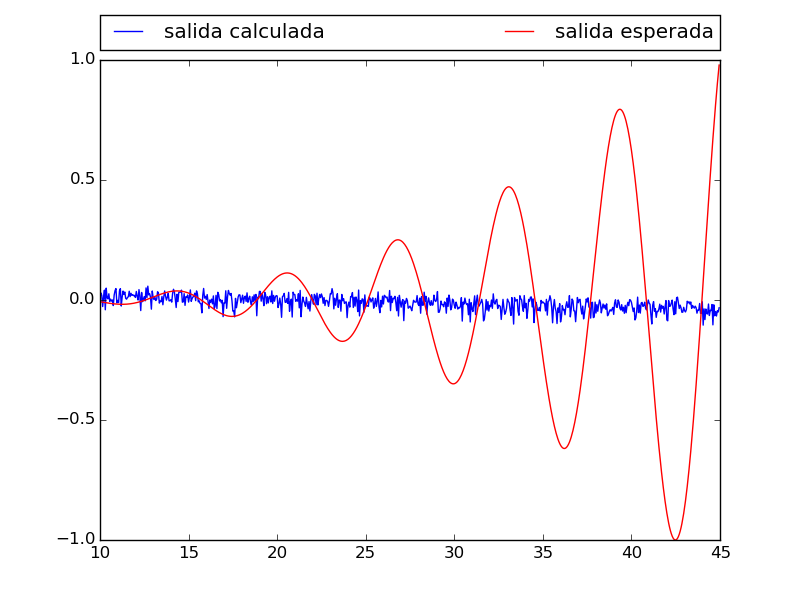
\includegraphics[width=0.85\textwidth]{img/_35_10-eta=0005-FUNCTION.png}
\caption{\label{fig:test5} Función. Datos:  $arq: 35-10, \acute{e} pocas \ =19000,\ \eta = 5 \times 10^{-3}, \ rango=(10, 45, 0.05),\ g=tanh, \ E = 1.21 \times 10^{-1}$}
\end{figure}

\begin{figure}[H]
\centering
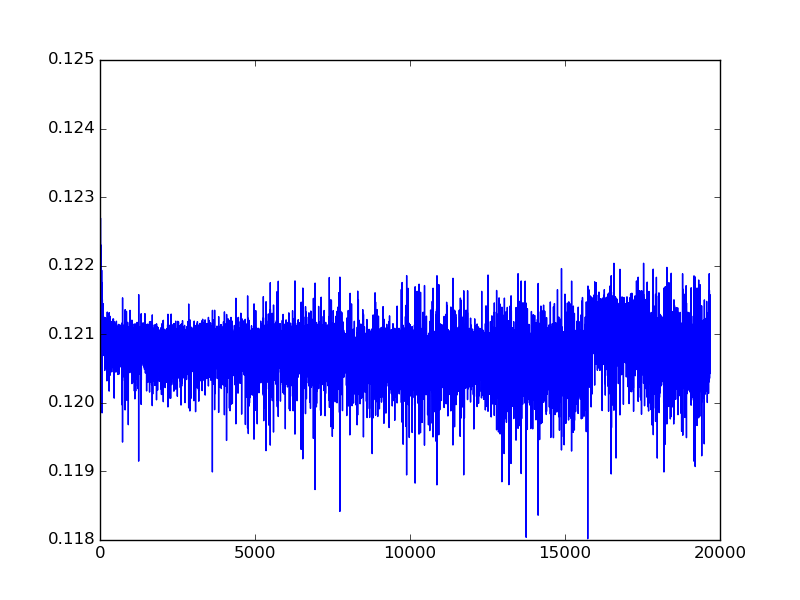
\includegraphics[width=0.85\textwidth]{img/_35_10-eta=0005-ERROR.png}
\caption{\label{fig:test5err} Error cuadrático medio. Datos:  $arq: 35-10, \acute{e} pocas \ =19000,\ \eta = 5 \times 10^{-3}, \ rango=(10, 45, 0.05),\ g=tanh, \ E = 1.21 \times 10^{-1}$}
\end{figure}

\begin{figure}[H]
\centering
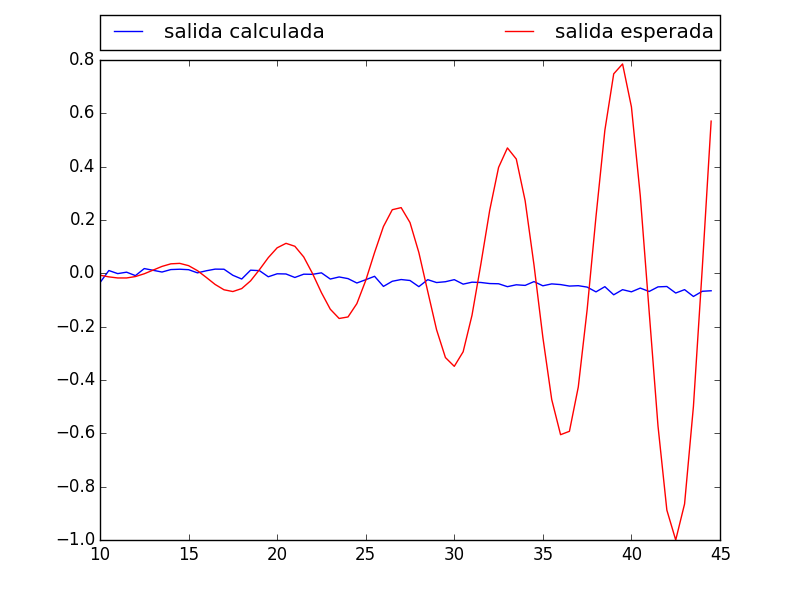
\includegraphics[width=0.85\textwidth]{img/_1024__512_-momentumadaptative-FUNCTION.png}
\caption{\label{fig:test10-45-momentum-adapt-fn} Función. Datos:  $arq: 1024-512, \acute{e} pocas \ = 23200,\ \eta \ adptativo, \ rango=(10, 45, 0.5),\ g=tanh, \ \alpha_{momentum} = 0.1, \alpha = 4 \times 10^{-4}, \ \beta = 0.5, \ E = 1.15 /times 10^{-1}$ }
\end{figure}

\begin{figure}[H]
\centering
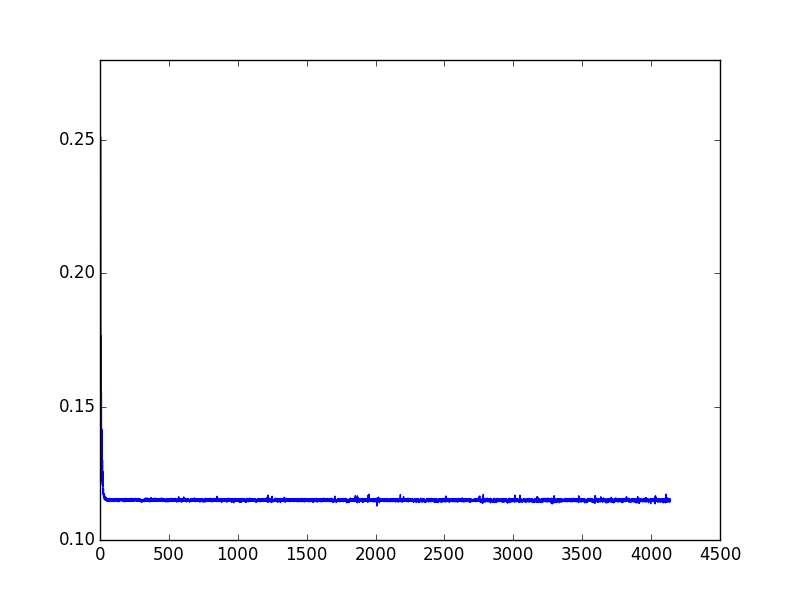
\includegraphics[width=0.85\textwidth]{img/_1024__512_-momentumadaptative-ERROR.png}
\caption{\label{fig:test10-45-momentum-adapt-error} Error cuadrático medio. Datos:  $arq: 1024-512, \acute{e} pocas \ = 23200,\ \eta \ adptativo, \ rango=(10, 45, 0.5),\ g=tanh, \ \alpha_{momentum} = 0.1, \alpha = 0.0004, \ \beta = 0.5, \ \beta_{fn \ act} = 1 \ E = 1.15 /times 10^{-1}$ }
\end{figure}

\begin{figure}[H]
\centering
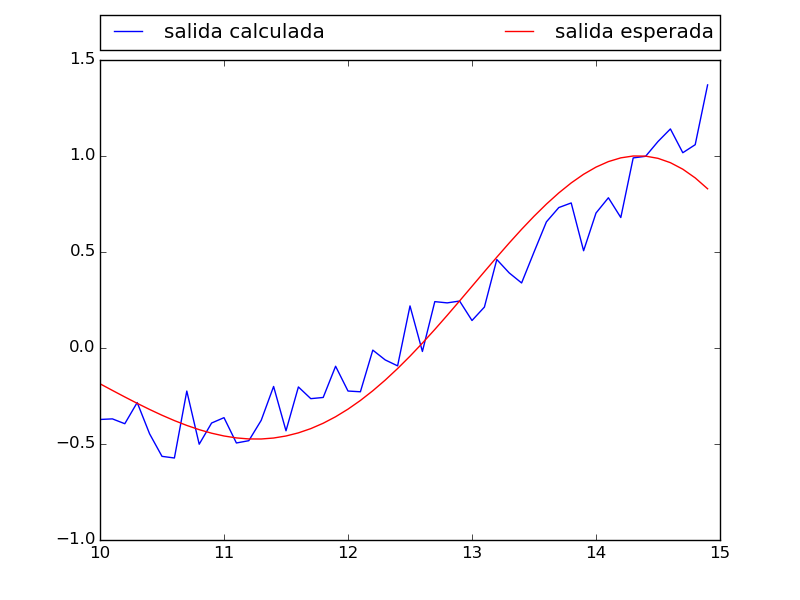
\includegraphics[width=0.85\textwidth]{img/_100_-eta_0_005-exp-FUNCTION.png}
\caption{\label{fig:test10-15-exp-fn-100} Función. Datos:  $arq: 100, \acute{e} pocas \ = 50000, \ \eta = 5 \times 10^{-3},\ rango=(10, 15, 0.1),\ g=exp, \ E = 3.17 \times 10^{-2}$}
\end{figure}


\begin{figure}[H]
\centering
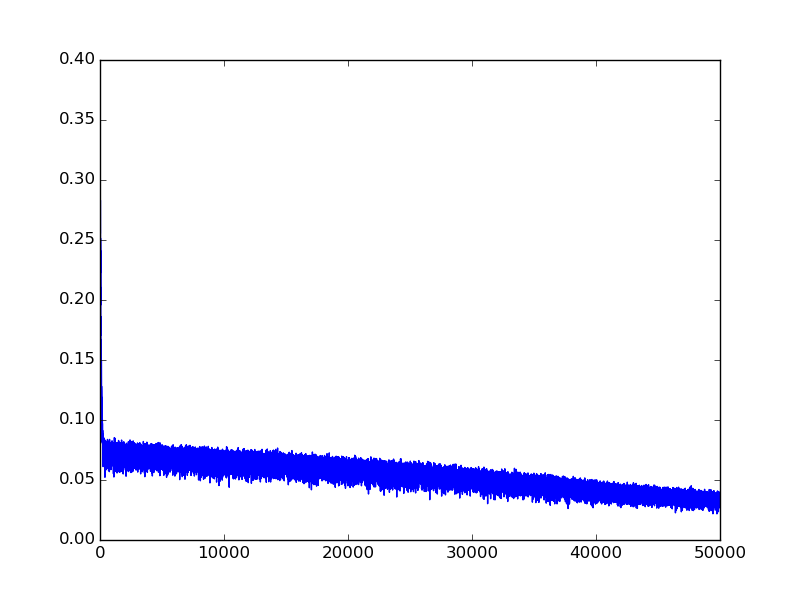
\includegraphics[width=0.85\textwidth]{img/_100_-eta_0_005-exp-ERROR.png}
\caption{\label{fig:test10-15-exp-error-100} Función. Datos:  $arq: 100, \acute{e} pocas \ = 50000, \ \eta = 5 \times 10^{-3},\ rango=(10, 15, 0.1),\ g=exp, \ E = 3.17 \times 10^{-2}$}
\end{figure}

\begin{figure}[H]
\centering
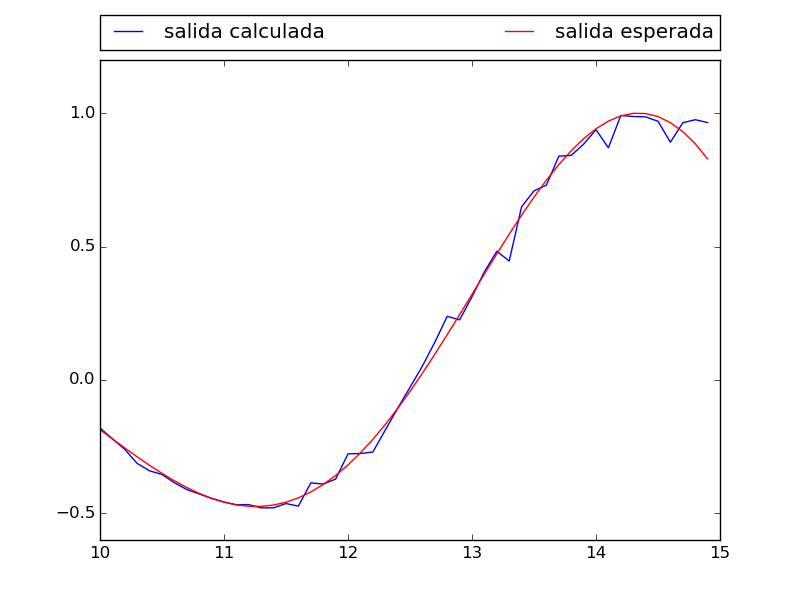
\includegraphics[width=0.85\textwidth]{img/_100_-eta_0_005-FUNCTION.png}
\caption{\label{fig:test10-15-tanh-fn-100} Función. Datos:  $arq: 100, \acute{e} pocas \ = 50000, \ \eta = 5 \times 10^{-3},\ rango=(10, 15, 0.1),\ g=exp, \ E = 1.48 \times 10^{-2}$}
\end{figure}

\begin{figure}[H]
\centering
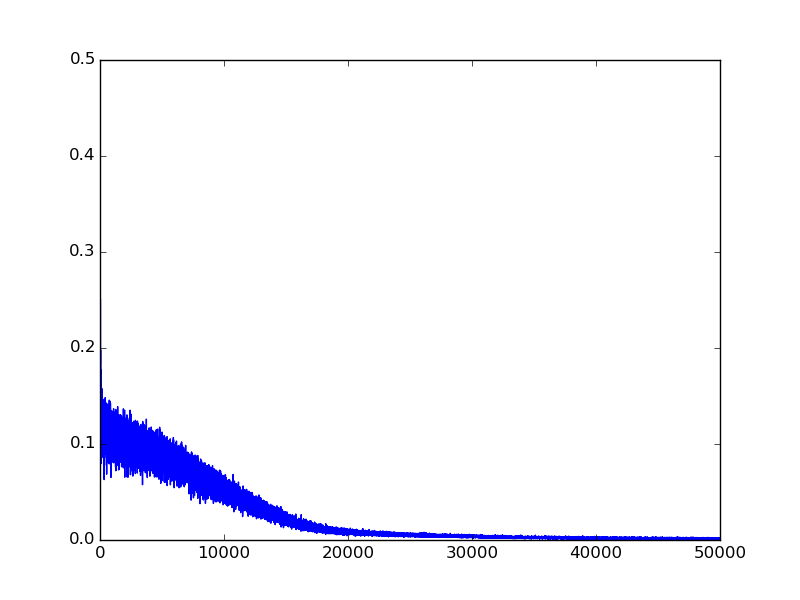
\includegraphics[width=0.85\textwidth]{img/_100_-eta_0_005-ERROR.png}
\caption{\label{fig:test10-15-tanh-error-100} Función. Datos:  $arq: 100, \acute{e} pocas \ = 50000, \ \eta = 5 \times 10^{-3},\ rango=(10, 15, 0.1),\ g=exp, \ E = 1.48 \times 10^{-2}$}
\end{figure}

\begin{figure}[H]
\centering
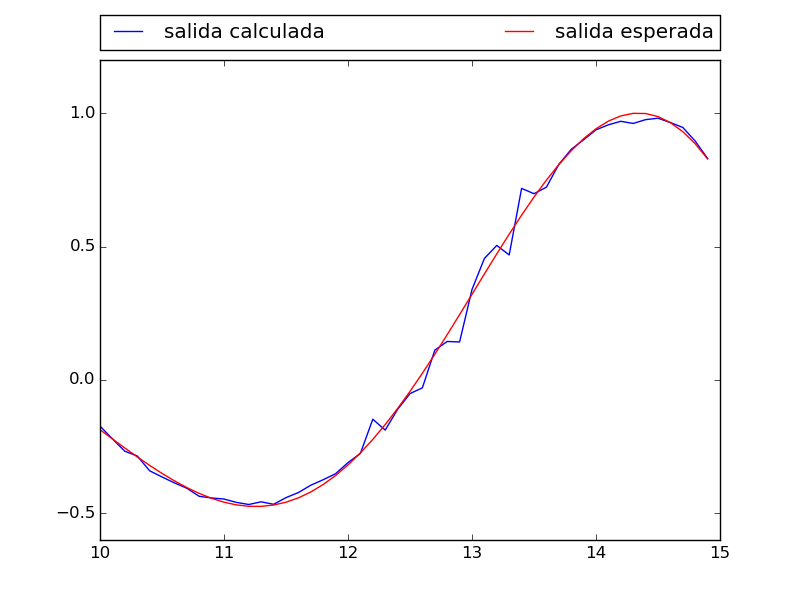
\includegraphics[width=0.85\textwidth]{img/_25__10_-eta_0_05-exp-FUNCTION.png}
\caption{\label{fig:test10-15-exp-fn-25} Función. Datos:  $arq: 25-10, \acute{e} pocas \ = 50000, \eta = 0.05,\ rango=(10, 15, 0.1),\ g=exp, \ E = 9.76 \times 10^{-4}$}
\end{figure}

\begin{figure}[H]
\centering
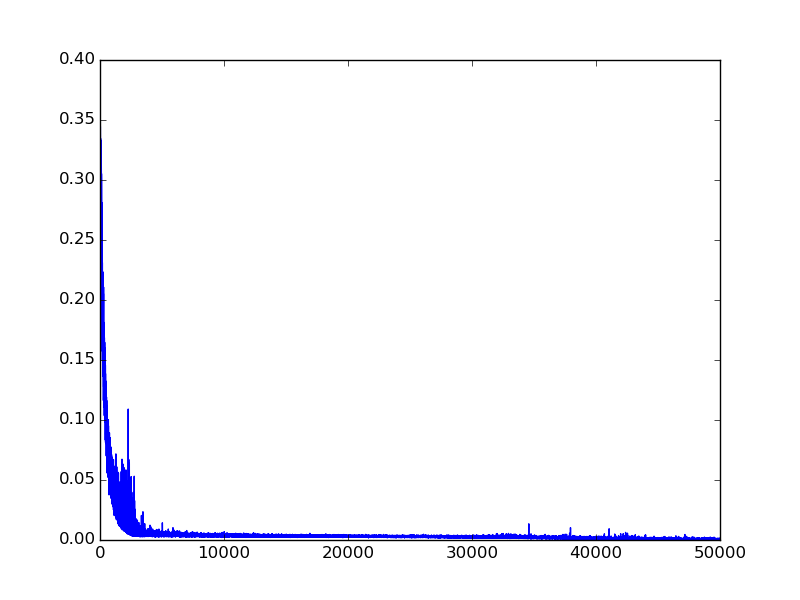
\includegraphics[width=0.85\textwidth]{img/_25__10_-eta_0_05-exp-ERROR.png}
\caption{\label{fig:test10-15-exp-error-25}  Error cuadrático medio. Datos:  $arq: 25-10, \acute{e} pocas \ = 50000, \eta = 0.05,\ rango=(10, 15, 0.1),\ g=exp, \ E = 9.76 \times 10^{-4}$}
\end{figure}

\begin{figure}[H]
\centering
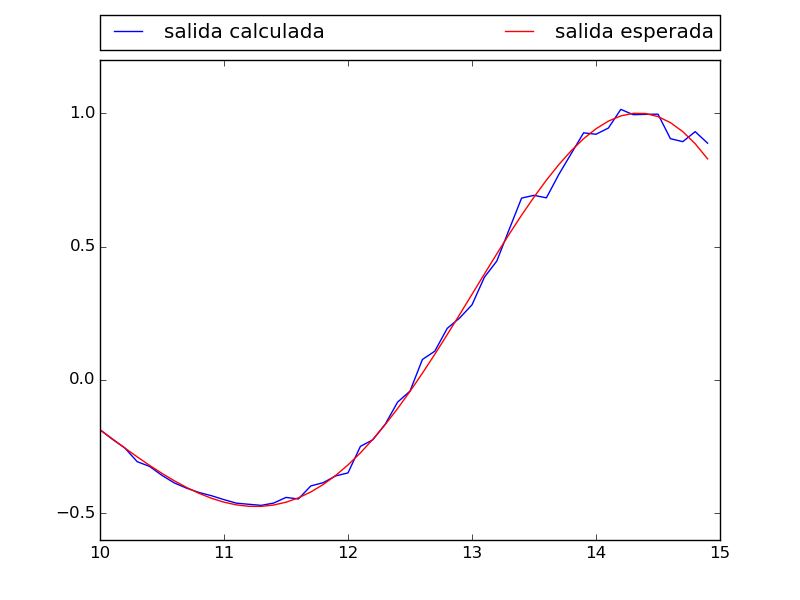
\includegraphics[width=0.85\textwidth]{img/_25__10_-eta_0_05-FUNCTION.png}
\caption{\label{fig:test10-15-tanh-fn-25} Función. Datos:  $arq: 25-10, \acute{e} pocas \ = 8605, \eta = 0.05,\ rango=(10, 15, 0.1),\ g=tanh, \ E = 9.21 x 10^{-5}$}
\end{figure}

\begin{figure}[H]
\centering
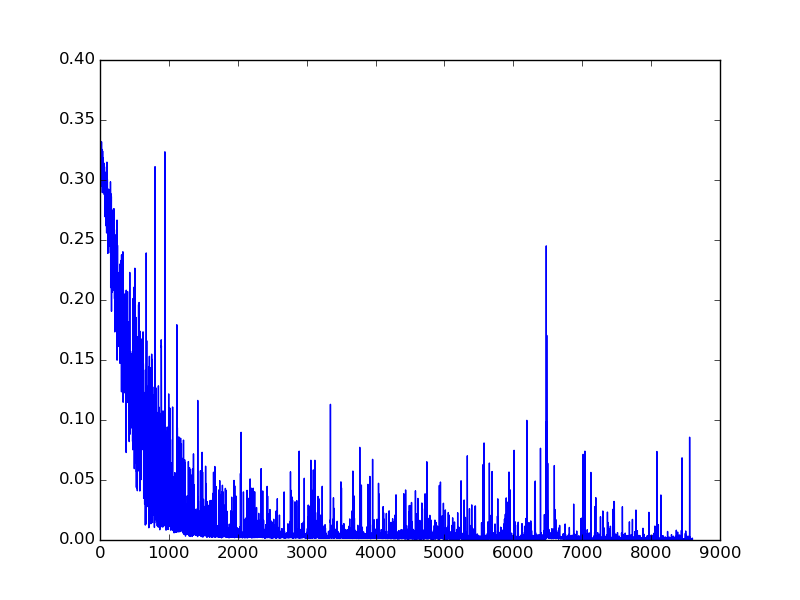
\includegraphics[width=0.85\textwidth]{img/_25__10_-eta_0_05-ERROR.png}
\caption{\label{fig:test10-15-tanh-error-25} Error cuadrático medio. Datos:  $arq: 25-10, \acute{e} pocas \ = 8605, \eta = 0.05,\ rango=(10, 15, 0.1),\ g=tanh, \ E = 9.21 \times 10^{-5}$}
\end{figure}

\begin{figure}[H]
\centering
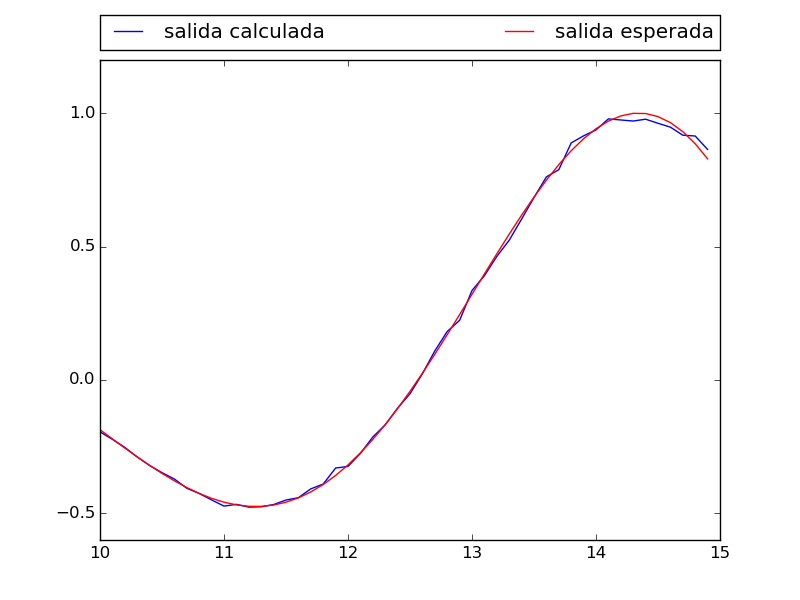
\includegraphics[width=0.85\textwidth]{img/_32__16__16_-eta_0_05-exp-FUNCTION.png}
\caption{\label{fig:test10-15-exp-fn-32} Función. Datos:  $arq: 32-16-16, \acute{e} pocas \ = 50000, \eta = 0.05,\ rango=(10, 15, 0.1),\ g=exp, \ E = 1.94 \times 10^{-4}$}
\end{figure}

\begin{figure}[H]
\centering
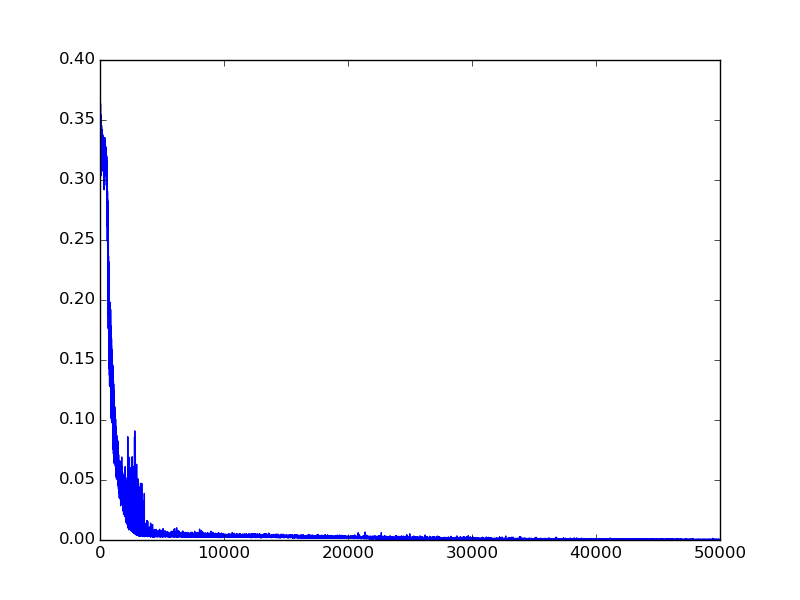
\includegraphics[width=0.85\textwidth]{img/_32__16__16_-eta_0_05-exp-ERROR.png}
\caption{\label{fig:test10-15-exp-error-32} Error cuadrático medio. Datos:  $arq: 32-16-16, \acute{e} pocas \ = 50000, \eta = 0.05,\ rango=(10, 15, 0.1),\ g=exp, \ E = 1.94 \times 10^{-4}$}
\end{figure}

\begin{figure}[H]
\centering
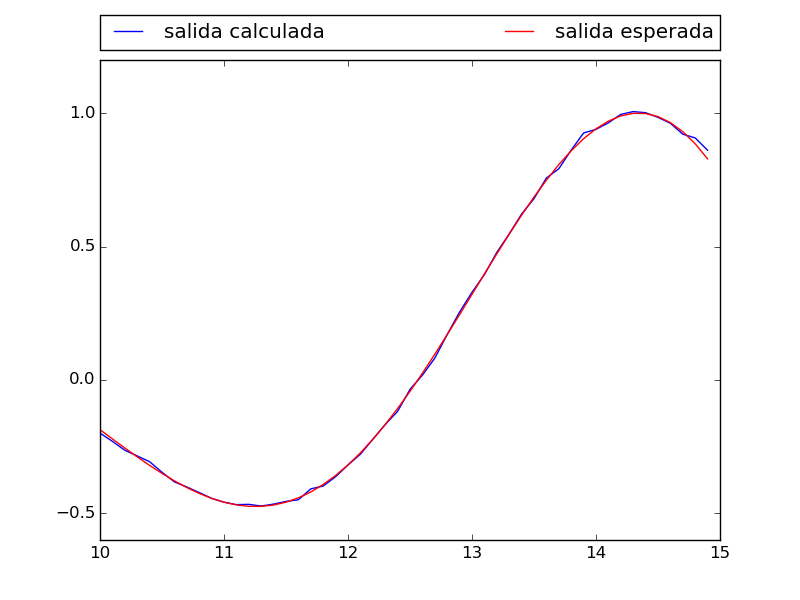
\includegraphics[width=0.85\textwidth]{img/_32__16__16_-eta_0_05-1430817237_7846918-FUNCTION.png}
\caption{\label{fig:test10-15-tanh-fn-32} Función. Datos:  $arq: 32-16-16, \acute{e} pocas \ = 4823, \ \eta = 0.05,\ rango=(10, 15, 0.1),\ g=tanh, \ E = 8,25 \times 10^{-5}$}
\end{figure}

\begin{figure}[H]
\centering
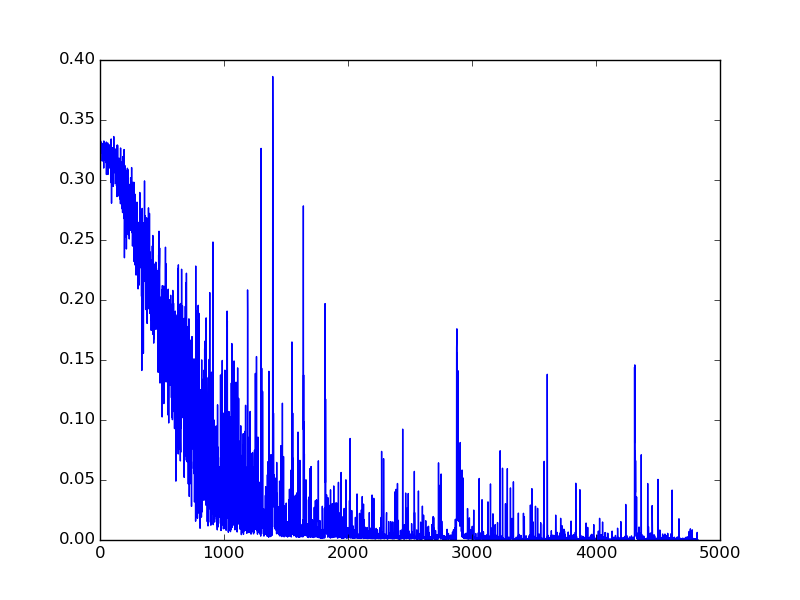
\includegraphics[width=0.85\textwidth]{img/_32__16__16_-eta_0_05-1430817237_7846918-ERROR.png}
\caption{\label{fig:test10-15-tanh-error-32} Error cuadrático medio. Datos:  $arq: 32-16-16, \acute{e} pocas \ = 4823, \ \eta = 0.05,\ rango=(10, 15, 0.1),\ g=tanh, \ E = 8,25 \times 10^{-5}$}
\end{figure}

\begin{figure}[H]
\centering
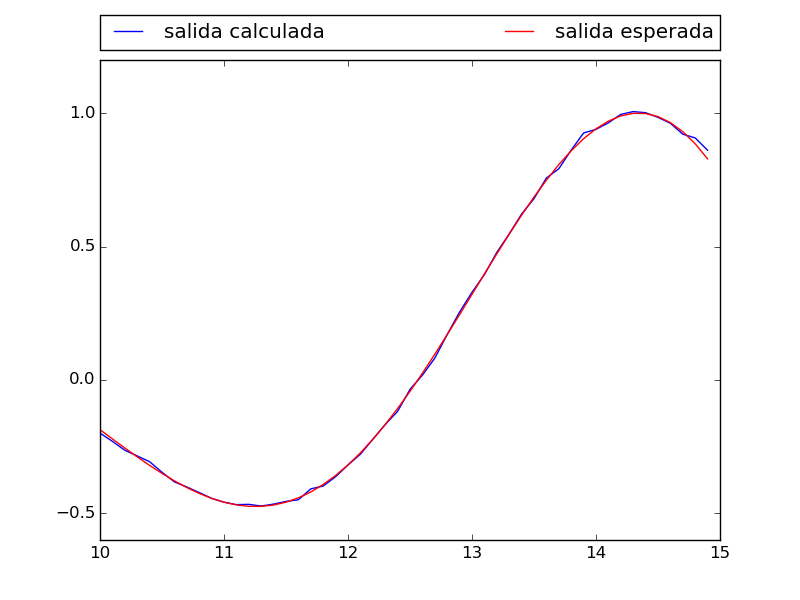
\includegraphics[width=0.85\textwidth]{img/_32__16__16_-eta_0_05-1430817237_7846918-FUNCTION.png}
\caption{\label{fig:test10-15-tanh-fn-32-momentum} Función. Datos:  $arq: 32-16-16, \acute{e} pocas \ = 3385, \ \eta = 0.05, \ \alpha_{momentum} = 0.3, \ rango=(10, 15, 0.1),\ g=tanh, \ E =9,32 \times 10^{-5}$}
\end{figure}

\begin{figure}[H]
\centering
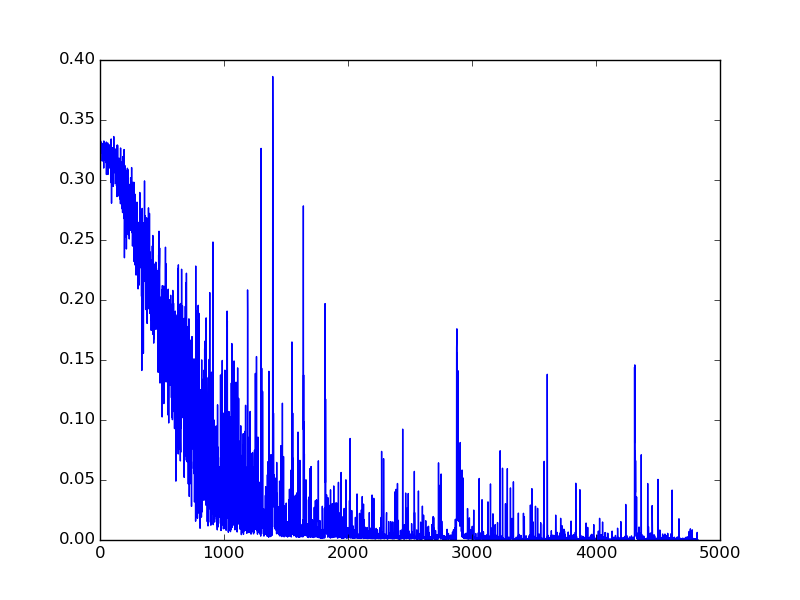
\includegraphics[width=0.85\textwidth]{img/_32__16__16_-eta_0_05-1430817237_7846918-ERROR.png}
\caption{\label{fig:test10-15-tanh-error-32-momentum} Error cuadrático medio. Datos:  $arq: 32-16-16, \acute{e} pocas \ = 3385, \ \eta = 0.05, \ \alpha_{momentum} = 0.3, \ rango=(10, 15, 0.1),\ g=tanh, \ E =9,32 x 10^{-5}$}
\end{figure}

\begin{figure}[H]
\centering
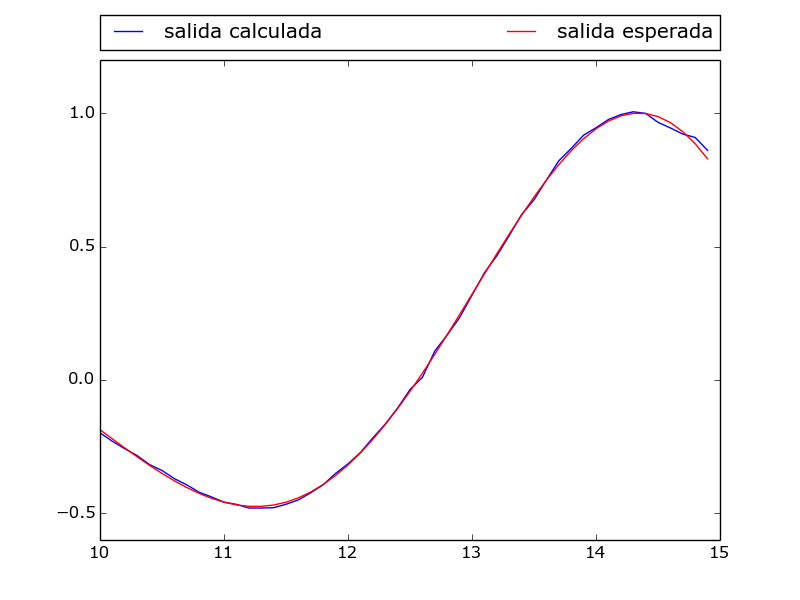
\includegraphics[width=0.85\textwidth]{img/_32__16__16_adaptative-1430833266_2379603-FUNCTION.png}
\caption{\label{fig:test10-15-tanh-fn-32-adaptative} Función. Datos:  $arq: 32-16-16, \acute{e} pocas \ = 3136, \ \eta \ adaptativo, \ \alpha = 4x10^{-3}, \ \beta =0.1  \ rango=(10, 15, 0.1),\ g=tanh, \ E =9,27 \times 10^{-5}$}
\end{figure}

\begin{figure}[H]
\centering
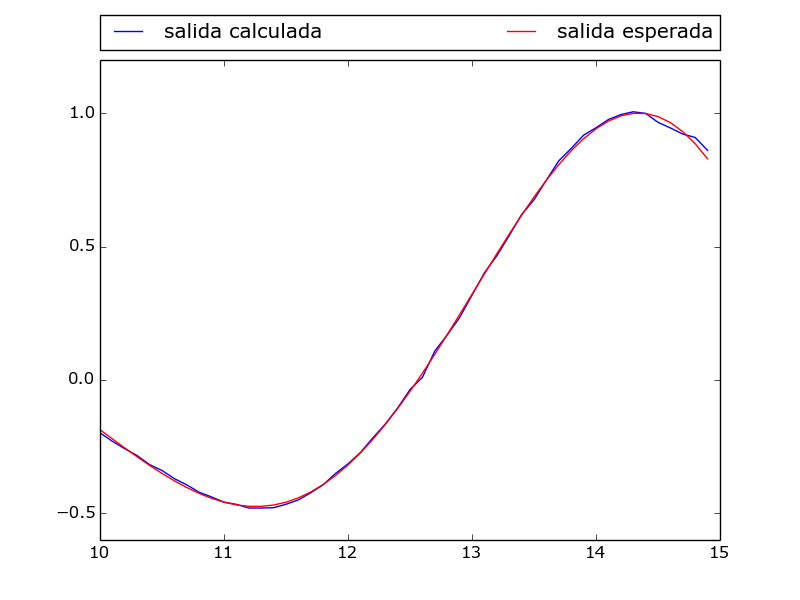
\includegraphics[width=0.85\textwidth]{img/_32__16__16_adaptative-1430833266_2379603-FUNCTION.png}
\caption{\label{fig:test10-15-tanh-error-32-adaptative}  Error cuadrático medio. Datos:  $arq: 32-16-16, \acute{e} pocas \ = 3136, \ \eta \ adaptativo, \ \alpha = 4x10^{-3},\ \beta =0.1  \ rango=(10, 15, 0.1),\ g=tanh, \ E =9,27 \times 10^{-5}$}
\end{figure}

\begin{figure}[H]
\centering
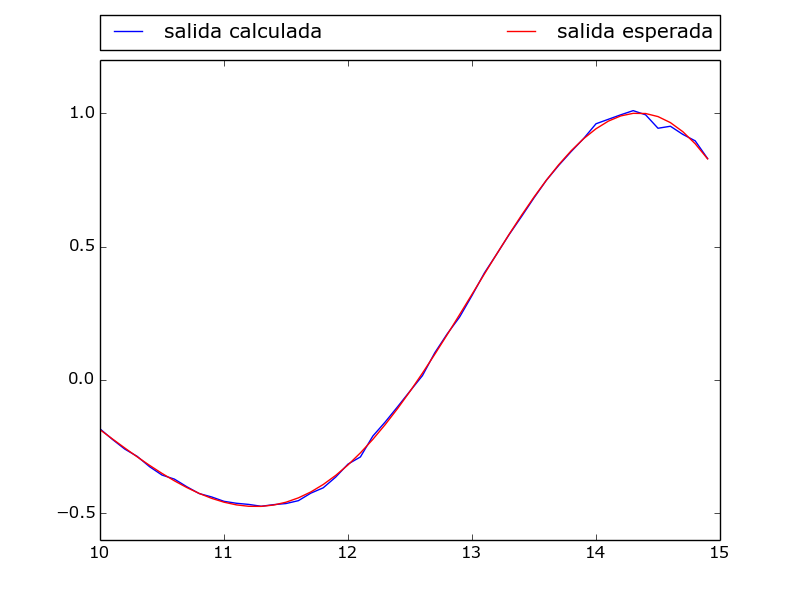
\includegraphics[width=0.85\textwidth]{img/_32__16__16_-momentumadaptative-1430834275_8048704-FUNCTION.png}
\caption{\label{fig:test10-15-tanh-fn-32-adaptative-momentum} Función. Datos:  $arq: 32-16-16, \acute{e} pocas \ = 3188, \ \eta \ adaptativo, \ \alpha_{momentum} = 0.3, \ \alpha = 4x10^{-3},\ \beta =0.1  \ rango=(10, 15, 0.1),\ g=tanh, \ E =8,64 \times 10^{-5}$}
\end{figure}

\begin{figure}[H]
\centering
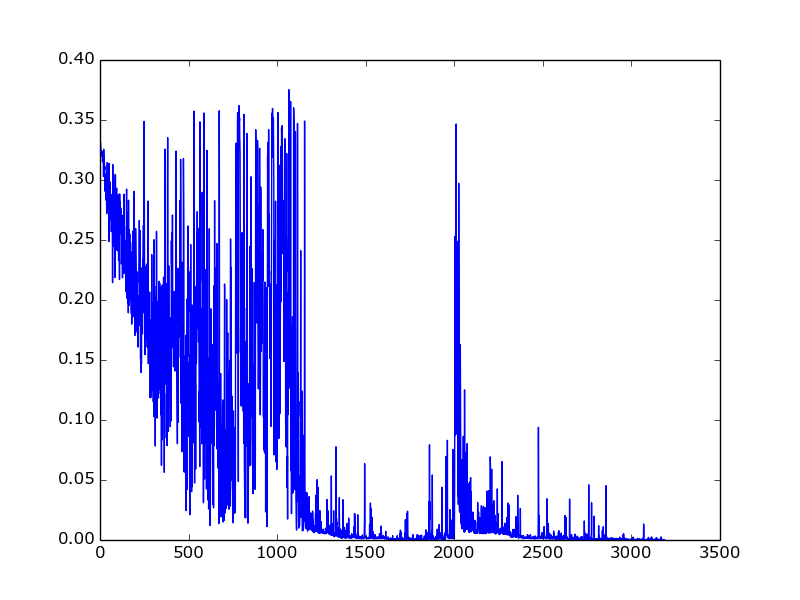
\includegraphics[width=0.85\textwidth]{img/_32__16__16_-momentumadaptative-1430834275_8048704-ERROR.png}
\caption{\label{fig:test10-15-tanh-error-32-adaptative-momentum} Función. Datos:  $arq: 32-16-16, \acute{e} pocas \ = 3188, \ \eta \ adaptativo, \ \alpha_{momentum} = 0.1, \ \alpha = 4x10^{-3},\ \beta =0.1  \ rango=(10, 15, 0.1),\ g=tanh, \ E =8,64 \times 10^{-5}$}
\end{figure}

\begin{figure}[H]
\centering
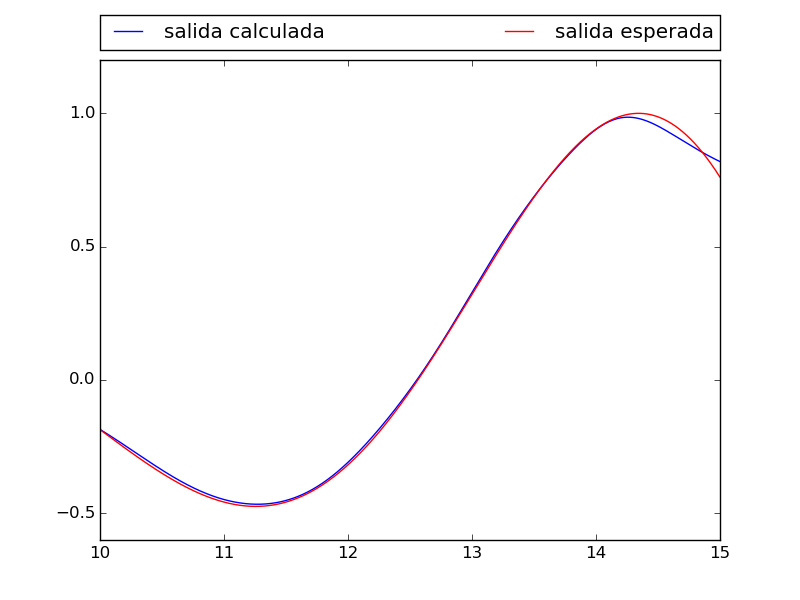
\includegraphics[width=0.85\textwidth]{img/_32_16_16_FUNCTION-0001.png}
\caption{\label{fig:test10-15-tanh-fn-32-0.001} Función. Datos:  $arq: 32-16-16, \acute{e} pocas \ = 4823, \ \eta = 0.05,\ rango=(10, 15, 0.001),\ g=tanh, \ E_{gen} = 8,29 x 10^{-5}$}
\end{figure}

\begin{figure}[H]
\centering
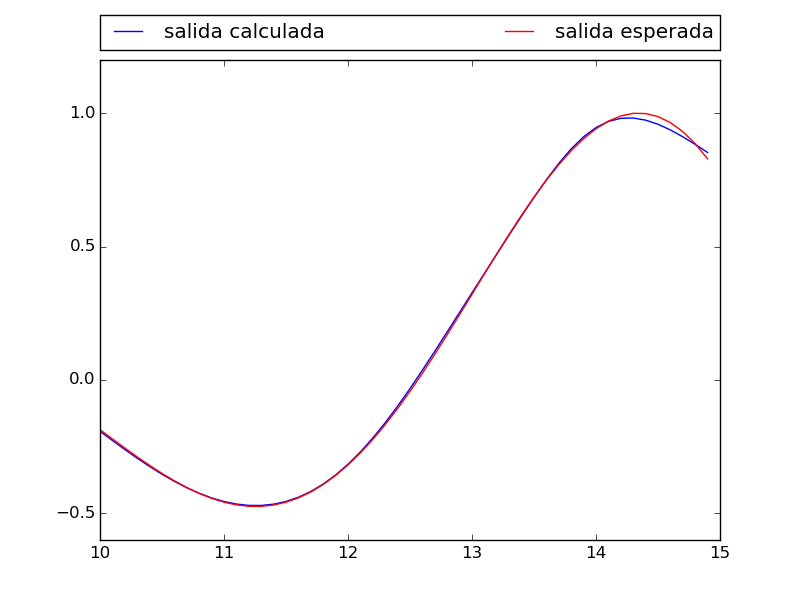
\includegraphics[width=0.85\textwidth]{img/_32_16_16-momentum0001.png}
\caption{\label{fig:test10-15-tanh-fn-32-momentum-0.001} Función. Datos:  $arq: 32-16-16, \acute{e} pocas \ = 3385, \ \eta = 0.05, \ \alpha_{momentum} = 0.3, \ rango=(10, 15, 0.001),\ g=tanh, \ E_{gen} =9,38 \times 10^{-5}$}
\end{figure}

\begin{figure}[H]
\centering
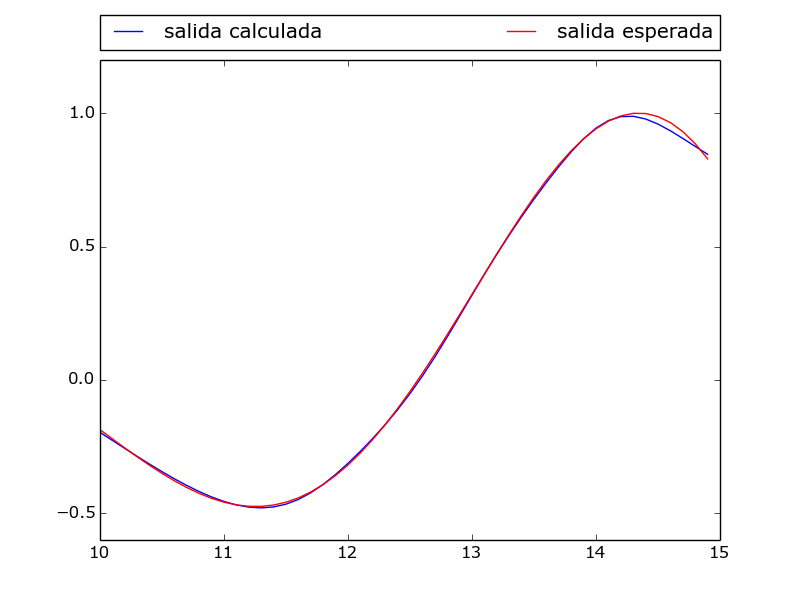
\includegraphics[width=0.85\textwidth]{img/_32__16__16_adaptative-test-1430833617_1787126-FUNCTION-0_001.png}
\caption{\label{fig:test10-15-tanh-fn-32-adaptative-0.001} Función. Datos:  $arq: 32-16-16, \acute{e} pocas \ = 3136, \ \eta \ adaptativo, \ \alpha = 4x10^{-3},\ \beta =0.1  \ rango=(10, 15, 0.001),\ g=tanh, \ E_{gen} =9,35 \times 10^{-5}$}
\end{figure}

\begin{figure}[H]
\centering
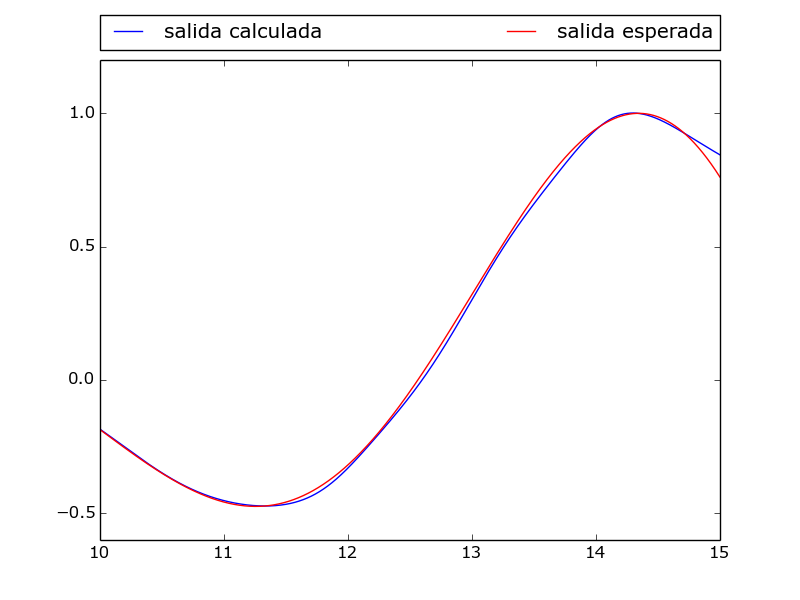
\includegraphics[width=0.85\textwidth]{img/_32__16__16_-momentumadaptative-test-1430834380_6222725-FUNCTION-0_001.png}
\caption{\label{fig:test10-15-tanh-fn-32-adaptative-momentum-0.001} Función. Datos:  $arq: 32-16-16, \acute{e} pocas \ = 3188, \ \eta \ adaptativo, \ \alpha_{momentum} = 0.3, \ \alpha = 4x10^{-3},\ \beta =0.1  \ rango=(10, 15, 0.1),\ g=tanh, \ E_{gen} =8,81 \times 10^{-5}$}
\end{figure}

\begin{figure}[H]
\centering
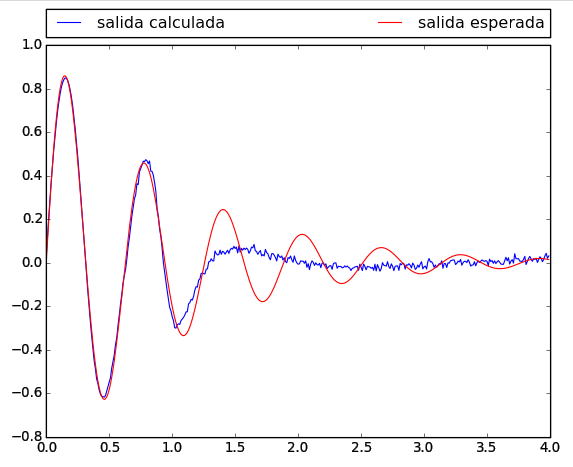
\includegraphics[width=0.85\textwidth]{img/ecuacion1.png}
\caption{\label{fig:ecuacion1} $y = sin(10x)e^{-x}\text{, con }  x \ \epsilon [-4,4]$. Datos: $arq: 10-5,\ \acute{e} pocas \ = 19200,\ rango=(0, 4, 0.1),\ g=tanh, \ E = 0.00603713708496,\ \eta = 10^{-3}$}
\end{figure}a

\begin{figure}[H]
\centering
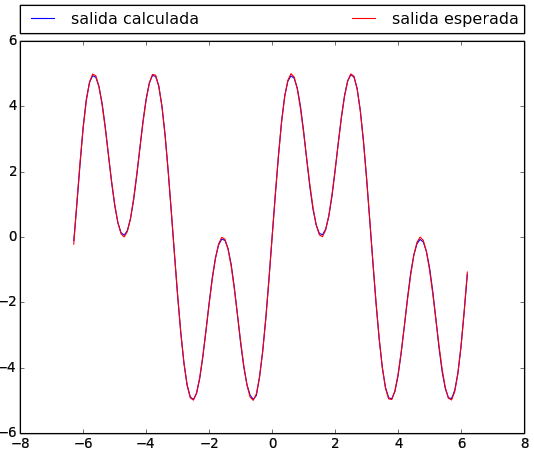
\includegraphics[width=0.85\textwidth]{img/ecuacion2.png}
\caption{\label{fig:ecuacion2} $y = 13sin(xcos^{2}(x)\text{, con }  x \ \epsilon [-6.3,6.3]$. Datos: $arq: 20-10,\ \acute{e} pocas \ = 56740,\ rango=(-6.3, 6.3, 0.1),\ g=tanh, \ E = 1.32 \times 10^{-4},\ \eta = 6.8\times 10^{-5}$}
\end{figure}

\begin{figure}[H]
\centering
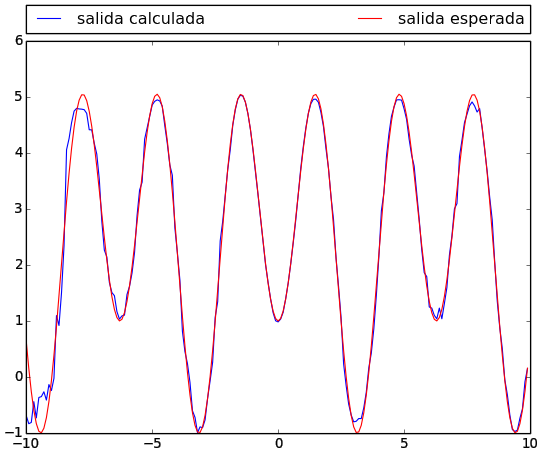
\includegraphics[width=0.85\textwidth]{img/ecuacion3.png}
\caption{\label{fig:ecuacion3} $y = 5sin^{2}(x) + cos(x)\text{, con }  x \ \epsilon [-10,10]$. Datos: $arq: 20-10,\ \acute{e} pocas \ = 20410,\ rango=(-10, 10, 0.1),\ g=tanh, \ E = 4.74 \times 10^{-2},\ \eta = 10^{-3}$}
\end{figure}

\begin{table}[H]
\centering
\hspace*{-1.5cm}
\begin{tabular}{|c|c|c|c|c|c|c|c|c|}
  \hline
  Arquitectura & $\eta$ & $fn$ & $\alpha$ & $\beta$ & $\alpha_{m}$ & épocas & $E_{ent}$ & $E_{gen(0.001)}$  \\
  \hline
  $100$ & $5\times 10^{-2}$ & $exp$ & $0$ & $0$ & $0$ & $50000$ & $3.34 \times 10^{-3}$ & $3.40 \times 10^{-2}$\\
  \hline
  $100$ & $5\times 10^{-2}$ & $tan$ & $0$ & $0$ & $0$ & $50000$ & $1.62 \times 10^{-3}$ & $1.74 \times 10^{-2}$\\
  \hline
  $25-10$ & $5\times 10^{-2}$ & $exp$ & $0$ & $0$ & $0$ & $50000$ & $9.91 \times 10^{-3}$ & $9.94 \times 10^{-3}$\\
  \hline
   $25-10$ & $5\times 10^{-2}$ & $tanh$ & $0$ & $0$ & $0$ & $8730$ & $9.33 \times 10^{-5}$ & $9.39 \times 10^{-5}$\\
  \hline
   $32-16-16$ & $5\times 10^{-2}$ & $exp$ & $0$ & $0$ & $0$ & $50000$ & $2.1 \times 10^{-4}$ & $2.15 \times 10^{-4}$\\
  \hline
   $32-16-16$ & $5\times 10^{-2}$ & $tanh$ & $0$ & $0$ & $0$ & $4915$ & $8.41 \times 10^{-5}$ & $8.49 \times 10^{-5}$\\
  \hline
  $32-16-16$ & $5\times 10^{-2}$ & $tanh$ & $0$ & $0$ & $0.3$ & $3560$ & $9.82 \times 10^{-5}$ & $9.94 \times 10^{-5}$\\
  \hline
  $32-16-16$ & $5\times 10^{-2}$ & $tanh$ & $4 \times 10^{-3}$ & $10^{-1}$ & $0$ & $3438$ & $9.90 \times 10^{-5}$ & $9.98 \times 10^{-5}$\\
  \hline
  $32-16-16$ & $5\times 10^{-2}$ & $tanh$ & $4 \times 10^{-3}$ & $10^{-1}$ & $0.3$ & $3244$ & $8.9 \times 10^{-5}$ & $9.12 \times 10^{-5}$\\
  \hline
\end{tabular}
\caption{Resultados promedio para el rango $(10,15,0.1)$. $E_{gen} = E$ generalizado, $E_{ent} = E $ entrenado}
\end{table}
\hspace*{-1.5cm}

\end{document}